\documentclass[a4paper,10pt]{article}
\usepackage[left=1in, right=1in, top=1in, bottom=1in]{geometry}
\usepackage{titlesec, xcolor, enumitem, hyperref, graphicx, tcolorbox, fontspec, multicol, setspace}
\usepackage{tikz}
\usepackage{fontawesome5}

% Set main font
\setmainfont{Noto Sans}[
    Kerning = On,
    Numbers = Uppercase, 
    BoldFont = Noto Sans SemiBold
]

% Formatting settings
\setlength\parindent{0pt}
\setstretch{1.3}
\setlength\columnsep{0.25in}
\pagestyle{empty}

% Define custom colors
\definecolor{darkblue}{RGB}{61,90,128}
\definecolor{lightblue}{RGB}{152,193,217}
\definecolor{main}{HTML}{5989cf} 
% Title format
\titleformat{\section}{\large\bfseries\color{darkblue}}{}{0em}{}[\titlerule]

% Hyperlink setup
\hypersetup{
    colorlinks=true,
    linkcolor=darkblue,
    urlcolor=darkblue,
}

% Custom Box Design
\tcbset{
    sharp corners,
    colback = white,
    before skip = 0.2cm,
    after skip = 0.5cm
}

% Profile Box
\newtcolorbox{boxM}{
    fontupper = \color{white},
    rounded corners,
    arc = 6pt,
    colback = darkblue, 
    colframe = darkblue, 
    boxrule = 0pt, 
    bottomrule = 4.5pt,
    enhanced
}

\newtcolorbox{boxB}{
    fontupper = \bf\color{main}, % font color
    boxrule = 1.5pt,
    colframe = main,
    rounded corners,
    arc = 5pt   % corners roundness
}

% Project Box
\newtcolorbox{projectbox}[2][]{colback=lightblue!5!white, colframe=lightblue!80!black, title=#2, fonttitle=\bfseries, coltitle=black}

\begin{document}

% Header
\begin{minipage}{0.65\textwidth}
    {\LARGE\bfseries Sudipta Singha Rathi}\\[0.5em]
    {\large Software Developer | Machine Learning Enthusiast}\\[0.5em]
    \faPhone \ +8801746-579065 \quad
    \faEnvelope \ \href{mailto:jucse29.408@gmail.com}{jucse29.408@gmail.com} \\
    \faGithub \ \href{https://github.com/sudiptarathi2020}{sudiptarathi2020} \quad
    \faLinkedin \ \href{https://linkedin.com/in/sudiptarathi2020}{LinkedIn}
\end{minipage}%
\hfill
\begin{minipage}{0.3\textwidth}
    \centering
    \begin{tikzpicture}
        \clip [rounded corners=0.5cm] (0,0) rectangle (3cm,3cm);
        \node at (1.5cm,1.5cm) {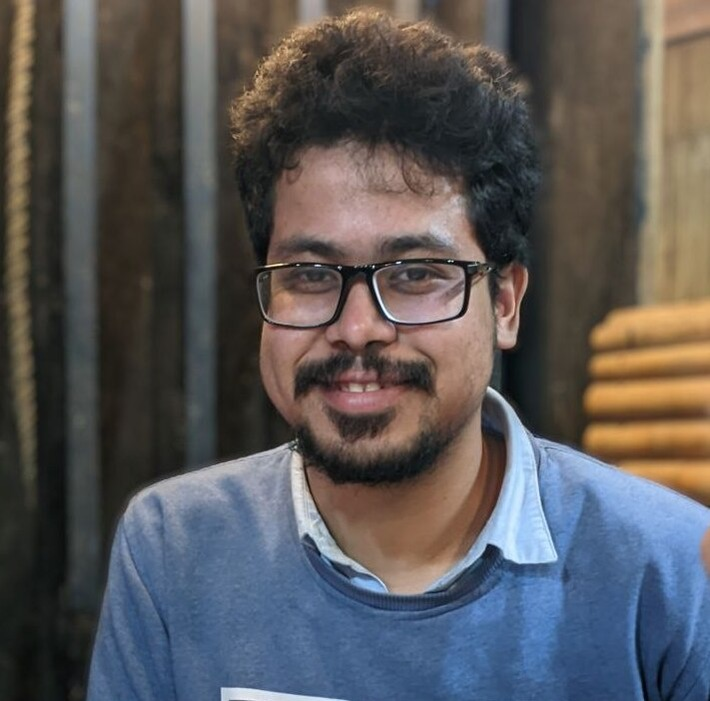
\includegraphics[width=3cm, height=3cm]{resources/profile.jpg}};
    \end{tikzpicture}
\end{minipage}

\vspace{1em}

% About Me
\section*{About Me}
A 4th-year Computer Science and Engineering student at Jahangirnagar University, passionate about Machine Learning, Reinforcement Learning, System Design, and DevOps.

% Education
\section*{Education}
\begin{itemize}[leftmargin=0.5cm]
    \item \textbf{Jahangirnagar University} – BSc in Computer Science and Engineering
    \item \textbf{Milestone College} – HSC in Science
    \item \textbf{Tetaigaon Rashid Uddin High School} – SSC in Science
\end{itemize}

% Skills
\section*{Skills}

\textbf{Programming:} Python, C, C++, Java, LaTeX, Bash \\
\textbf{Frameworks:} Django \\
\textbf{Tools:} Linux, Git, WSL, Docker, AWS \\
\textbf{Databases:} SQLite


% Projects
\section*{Projects}
\href{https://github.com/sudiptarathi2020/JUMCMS-Jahangirnagar-University-Medical-Center-Management-System.git}{\textbf{JUMCMS}}
\begin{boxB}
    A Django-based medical center management system for Jahangirnagar University, featuring appointment scheduling and medical records management.
\end{boxB}


\href{https://github.com/sudiptarathi2020/Software-Engineering-Lab-CSE404-Reports.git}{\textbf{Software Engineering Lab Reports}}
\begin{boxB}
A collection of software engineering lab reports documenting various projects and experiments.
\end{boxB}
\href{https://github.com/sudiptarathi2020/Data-structures-and-Algorithms.git}{\textbf{Data Structures \& Algorithms}}
\begin{boxB}
Templates and implementations of various data structures, algorithms, and problem-solving techniques.
\end{boxB}
\href{https://github.com/sudiptarathi2020/Simple-Chess-Engine.git}{\textbf{Chess Engine}}
\begin{boxB}
A chess engine using the minimax algorithm with alpha-beta pruning for intelligent move selection.
\end{boxB}
\href{https://github.com/sudiptarathi2020/academic-report-maker.git}{\textbf{Academic Report Maker}}
\begin{boxB}
A Django + React web application for generating academic reports with structured formatting.
\end{boxB}
\href{https://github.com/sudiptarathi2020/Problem-Solves.git}{\textbf{Online Judge Problem Solutions}}
\begin{boxB}
Solutions to problems from Codeforces, LightOJ, and other online judges, with explanations.
\end{boxB}

% Online Judge Statistics
\section*{Online Judge Statistics}
\begin{multicols}{2}
\textbf{Codeforces:} 500+ problems solved \\
\textbf{LightOJ:} 300+ problems solved \\
\textbf{HackerRank:} 100+ problems solved \\
\textbf{LeetCode:} 150+ problems solved
\end{multicols}

\end{document}
